\documentclass[final,3p,times,twocolumn]{elsarticle}
\usepackage{amsmath,amssymb,graphicx,booktabs,multirow,url}
\graphicspath{{figures/}}
\newenvironment{widefigure}[1][t]{\begin{figure*}[#1]}{\end{figure*}}
\newenvironment{widetable}[1][t]{\begin{table*}[#1]}{\end{table*}}
\newcommand{\myna}{\textsc{Myna}}
\newcommand{\stream}{\textsc{Myna-Stream}}
\newcommand{\vsix}{\textsc{Myna-v6}}
\journal{Elsevier}
\begin{document}
\begin{frontmatter}
\title{Myna: Cardinality-Aware Routing, Bundle Consistency, and Conformal Abstention for Non-Autoregressive Agent Decision Engines}
\author[1]{Aashish Kumar Mahato}
\affiliation[1]{organization={Independent Researcher}, city={Kathmandu}, country={Nepal}}
\tnotetext[1]{Graduate of Vellore Institute of Technology (VIT), Vellore, India. This work was conducted independently after graduation.}
\begin{abstract}
Agent loops make many small typed decisions over states that grow. A non-autoregressive decision engine answers such questions by scoring a fixed option set instead of generating text. We study three failure modes of this design on a frozen 16-cell suite: accuracy collapse when many options are packed into one sequence, logical inconsistency across the questions of a bundle, and uncalibrated confidence. We report \myna, two engines behind one typed \texttt{choice}/\texttt{score}/\texttt{noul} contract: a 14.45M gated-linear-attention streaming engine with a 576 KiB state, and a 446.63M fine-tuned DeBERTa-v3-large with cardinality-routed readout. Routing questions with more than 16 options to decoupled scoring repairs the 77-way banking77 cell from 0.0086 to 0.5345 and lifts 16-cell macro by 0.0329, while the other 15 cells remain identical. The accuracy arm reaches 0.8583 macro (our re-score is 0.8620, 95\% CI [0.8430, 0.8800]) and 83.76\% joint bundle exact match. Under an explicit entailment predicate we measure 3/172 contradictions, not the 0/172 the checkpoint records; the campaign's predicate is not released. Calibration is good (ECE 0.0189, Brier 0.0434), but 90\% conformal sets cover only 85.49\%, so we do not claim coverage. The streaming arm answers in 33--870 ms, runs in a browser at $1.03\times10^{-6}$ probability drift, and is not the accuracy arm. The contribution is a measurement discipline: every claim carries its arm, its denominator, and what it does not license.
\end{abstract}
\begin{keyword}
Decision engines \sep non-autoregressive inference \sep gated linear attention \sep cardinality routing \sep calibration \sep conformal prediction \sep selective prediction \sep edge deployment
\end{keyword}
\end{frontmatter}
\section{Introduction}
\label{sec:intro}

An agent that processes tickets, threads, or page states asks many small questions: is this a refund request, how severe is it, which department owns it. Each question has a small, fixed answer set, and the state on which it is asked grows with every turn. Autoregressive language models answer such questions fluently but pay for generation on every call and can return text outside the option set. A non-autoregressive \emph{decision engine} instead returns a categorical distribution over predefined options \cite{li2026jev,duan2026gdm}. The design is attractive for high-frequency routing, but three things can go wrong, and all three are measurable.

First, \textbf{option cardinality is a budget}. A single sequence that carries a question, a state, and every option competes for one fixed window. On a 77-way intent question the option spans alone consume almost the whole window, and a packed model can fall to near chance even though it is accurate on 4-way questions. Second, \textbf{a bundle can contradict itself}: a model may call an article “sports” and then answer “no” to “is this sports?”. Third, \textbf{confidence can be miscalibrated}, and an abstention rule built on it can withhold the wrong answers.

This paper studies those three failure modes on \textsc{decision-v2-pilot}, a frozen suite of 1{,}176 bundles and 1{,}440 questions over 16 cells and 11 public sources (Table~\ref{tab:dataset}). We report \myna, which is not one model but two engines behind one typed contract. \stream{} is a 14.45M-parameter gated-linear-attention engine whose retained state is 576 KiB at every length from 128 to 16{,}384 tokens; it scans a state once and answers later questions from the cache. \vsix{} is a 446.63M-parameter fine-tuned DeBERTa-v3-large with a cardinality-routed readout; it re-encodes the state on every ask and is the accuracy arm. The two share the question schema, the answer record, the abstention seam, and the serving API, and nothing else. Keeping them separate is the first methodological decision of the paper: a speed number from \stream{} is not a statement about \vsix{}, and an accuracy number from \vsix{} is not a statement about \stream{}.

\textbf{Scope.} This is a single-system study. Every comparison in the paper is an internal ablation on the same frozen suite; we do not report head-to-head numbers against external engines. The v6 arm is fine-tuned in-domain on the suite, so its accuracy is a measurement of that arm, not a claim about out-of-domain generalization. The paper's contribution is the measurement protocol and the artifacts that make each number checkable, not a leaderboard position.

Our contributions are four measurements and one negative mechanism result.
\begin{itemize}
\item \textbf{A cardinality diagnosis and a routing fix.} We measure the token budget of the packed layout on every cell. All questions with $K\le15$ options fit with zero dropped options; the 77-way cell overflows on 50 of 116 rows, consumes 490 option-span tokens (6.36 tokens per option), and scores 0.0086. Routing $K>16$ to decoupled per-option scoring raises that cell to 0.5345 (v5) and 0.6638 (v6), and lifts 16-cell macro by 0.0329 and 0.0081 respectively. The other 15 cells are byte-identical at a macro of 0.8712; the gain is one cell, and we say so.
\item \textbf{A reproducible bundle-consistency measurement.} The checkpoint records 0/172 contradictions, but the predicate that produced it is not in the repository. We define an explicit entailment predicate, re-score the same 172 bundles, and measure 3/172 for \vsix{}. The cross-question graph module in the checkpoint is inert at inference, so consistency is a property of the fine-tuned encoder, not an enforced constraint.
\item \textbf{A calibration and abstention audit.} Per-primitive temperature scaling gives ECE 0.0189 and Brier 0.0434 with zero argmax flips between dev and test. Selective accuracy at 60\% coverage is 98.73\% as reported (98.15\% under our re-ranking). But split-conformal 90\% sets cover 85.49\% of test questions, not 90\%, and 95\% sets cover 93.68\%; we report the undercoverage and treat the sets as a ranking signal rather than a coverage certificate.
\item \textbf{A systems study of the streaming arm.} On one Apple M5, \stream{} answers 33.08 ms at one question and 869.95 ms at fifty end-to-end, with a 576 KiB state that does not grow. It runs under MLX at 1.76--2.22$\times$ over PyTorch MPS and in Chrome/WebAssembly at 59.32 MiB and $1.03\times10^{-6}$ maximum probability drift. int8 is 3.17$\times$ smaller but not faster and not faithful (6.48e-2 drift in ONNX, one argmax flip in MLX), so fp32 ships.
\item \textbf{A negative result about the small engine.} The same architecture trained from scratch on this suite plateaus at 0.4893--0.5339, and its long-context arm is flat at chance (0.183 at 4k, 0.150 at 16k). Removing a majority-label shortcut eliminates four constant-emitter cells but costs 0.0554 macro. The gap to the fine-tuned arm is a representation gap, not a dose we can fix by training longer, and the paper does not claim otherwise.
\end{itemize}

\section{Related Work}
\label{sec:related}

\paragraph{Typed and zero-shot decision models.}
Cloze-style reformulation turns classification into scoring option strings \cite{schick2021pet}, and prompt-based fine-tuning with demonstrations improves few-shot performance \cite{gao2021lmbff}. Entailment-based zero-shot classification scores labels as hypotheses \cite{yin2019benchmarking}; SetFit shows that sentence-encoder fine-tuning is competitive with prompts at small label budgets \cite{tunstall2022setfit}. The recent \emph{Jev} line makes the decision-model framing explicit: a model returns a categorical distribution over predefined options without generating text \cite{li2026jev}, and JEVal benchmarks that family across 36 datasets \cite{duan2026gdm}. JEVal's findings motivate our second and third failure modes: decision models can identify the likely outcome while substantially overstating its probability, and their errors compound in multi-step systems. Our suite is smaller and our arm is in-domain, but the failure modes are the same.

\paragraph{Efficient sequence models.}
Linear attention replaces the quadratic attention matrix with a recurrence whose state is fixed in size \cite{katharopoulos2020transformers}; gated linear attention adds a data-dependent forget gate and hardware-efficient training \cite{yang2024gla}. State-space models such as Mamba \cite{gu2024mamba} and RWKV \cite{peng2023rwkv} make the same trade, and IO-aware exact attention \cite{dao2022flashattention} and sparse attention \cite{beltagy2020longformer} attack the cost from other directions. Our streaming arm is a six-layer gated-linear-attention trunk; the citation here is lineage and motive, not a claim that the trunk is a new architecture.

\paragraph{Calibration, selective prediction, and conformal sets.}
Temperature scaling and reliability diagrams are the standard calibration tools \cite{guo2017calibration}; modern networks remain miscalibrated under dataset shift \cite{ovadia2019uncertainty}. Selective classification trades coverage for risk \cite{geifman2017selective,geifman2019selectivenet}. Split conformal prediction gives distribution-free marginal coverage under exchangeability \cite{lei2018distribution,angelopoulos2021gentle}, and conformalized quantile regression reports coverage and interval length together \cite{romano2019cqr}. We follow the reporting convention, not the guarantee: our empirical coverage is below nominal, and we say so.

\paragraph{Consistency and structured readout.}
Semantic loss injects logical constraints into training \cite{xu2018semantic}; self-consistency samples multiple reasoning paths and votes \cite{wang2023selfconsistency}; guided generation constrains decoding with a finite-state machine \cite{willard2023guided}. Our setting differs: the readout is a single forward pass per question, so there is no sampling to vote over and no decoder to constrain. We measure cross-question entailment after the fact, and we report that the checkpoint's graph module does not participate in inference.

\paragraph{Cascades, edge deployment, and quantization.}
Early-exit networks decide per input how much computation to spend \cite{teerapittayanon2016branchynet,xin2020fastbert,zhou2020deebert}. Post-training quantization reduces bytes but can move probabilities \cite{dettmers2022llmint8,frantar2023gptq,xiao2023smoothquant}. Our two-engine design is a coarse cascade: the constant-state engine handles frequent decisions and the cross-encoder is the accuracy arm; we measure the two ends and the portability of the small end, not a joint deferral policy.

\section{The Decision Contract and Two Engines}
\label{sec:contract}

\subsection{The typed contract}
A \emph{bundle} is a state $x$ and a set of questions $Q=\{q_1,\dots,q_m\}$. Each question has a type $\tau\in\{\texttt{choice},\texttt{score},\texttt{noul}\}$ and an option set $O_q$ with cardinality $K_q=|O_q|$. A \texttt{choice} returns one option; a \texttt{score} returns a level and an expected score; a \texttt{noul} returns $p(\text{yes})$. Every answer carries a probability vector, a confidence, a 90\% conformal set, an abstention flag, and the routing mode that produced it. The contract is the same for both engines; only the scorer behind it changes.

\subsection{\stream{}: constant state}
\stream{} is a six-layer gated-linear-attention trunk with $d_{\text{model}}=384$ and 14{,}449{,}280 parameters. An observation is scanned once into a per-layer state $S\in\mathbb{R}^{H\times d_k\times d_v}$; at production width this is 589{,}824 bytes (576 KiB), independent of the observation length. \texttt{observe()} scans, \texttt{append()} scans only the new segment, and \texttt{ask()} reads the question against $S$ with a pointer head. There is no vocabulary head and no LM trunk. The engine is the one that earns the phrase “never re-reads”.

\subsection{\vsix{}: cardinality-routed cross-encoder}
\vsix{} is a fine-tuned \texttt{microsoft/deberta-v3-large} (434{,}012{,}160 parameters, 24 layers, 512-token maximum) with 12{,}619{,}022 parameters of readout, for 446{,}631{,}182 total. It keeps four heads: a packed scorer, a set-aware head for high-cardinality questions, a CORAL ordinal head that the shipped config disables, and a cross-question graph module that inference never calls. For $K\le16$ it builds one packed sequence: a task prefix, the state, then each option followed by its own \texttt{[MASK]} token; the scorer reads the hidden state at each mask. For $K>16$ it encodes each option against the state separately and scores it against the competition in its bundle. The state is truncated before the options are, because dropping context degrades one shared span while dropping an option deletes a candidate; when the option spans themselves overflow, the tail is cut, which is exactly the v5 failure we diagnose in Section~\ref{sec:cardinality}. The engine re-encodes the whole state on every ask; it has no fixed-size state and no streaming property.

\subsection{What is shared, and what is not}
Both engines implement the same \texttt{observe}/\texttt{append}/\texttt{ask} surface, the same answer record, and the same fallback seam. \texttt{myna.serve} exposes \texttt{/v1/sessions} for either. The abstention rule is shared: an answer is withheld when the conformal set is empty or when the top probability is below a settable floor. The fallback records which engine committed, so a two-tier pipeline is auditable. What is not shared is the property that motivated the project: \stream{} has a constant state and \vsix{} does not. Figure~\ref{fig:arch} draws the two arms side by side; Table~\ref{tab:dataset} lists the suite.

\begin{widefigure}
\centering
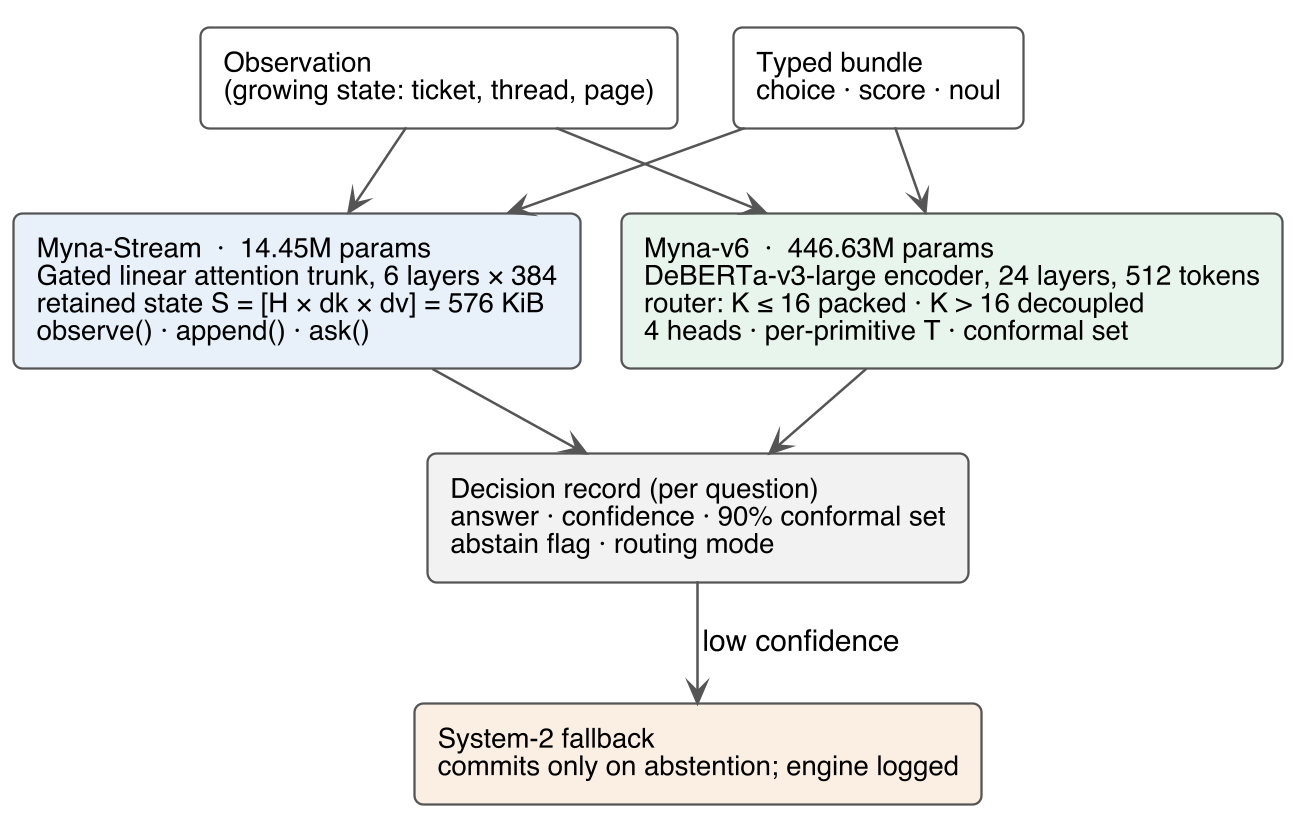
\includegraphics[width=0.82\linewidth]{fig1_architecture.png}
\caption{The two \myna{} engines behind one typed contract. \stream{} scans a growing observation once into a 576 KiB state and answers from the cache; \vsix{} re-encodes the state on every ask and routes by option cardinality. Both write the same decision record, and a low-confidence answer can be deferred to a System-2 engine with the committing engine logged. The figure is a schematic; the measurements are in Section~\ref{sec:systems}.}
\label{fig:arch}
\end{widefigure}

\begin{table}[t]
\centering
\footnotesize
\caption{The frozen \textsc{decision-v2-pilot} suite (11 public sources). Cells are the 16 $(\text{source},\text{question})$ pairs; $K$ is the number of options per question.}
\label{tab:dataset}
\begin{tabular}{lrrrr}
\toprule
Split & Rows & Questions & Cells & $K$ \\
\midrule
Train & 57{,}904 & 73{,}804 & 16 & 2--77 \\
Development & 1{,}176 & 1{,}440 & 16 & 2--78 \\
Calibration & 448 & 568 & 16 & 2--77 \\
Test & 1{,}176 & 1{,}440 & 16 & 2--78 \\
\bottomrule
\end{tabular}
\end{table}

\section{Cardinality Is a Budget}
\label{sec:cardinality}

\subsection{The packed layout and its failure}
The packed scorer spends one sequence on the prefix, the state, and all option spans. Each span is the option text, one \texttt{[MASK]}, and a separator. The state is truncated first, and if the option spans still exceed the window, the fallback keeps a prefix of the options and collapses the context to a single token. That fallback is not a graceful degradation: it deletes the state and the tail options at the same time.

We measured the budget on every test cell with the suite's own renderer and tokenizer (Figure~\ref{fig:cardinality}a). The 15 non-banking77 cells have $K=2$--$15$; none overflows, and every option gets a mask. The 77-way banking77 cell is different: mean option-span length is 490.3 tokens, or 6.36 tokens per option; with a median 25-token state, the total exceeds 512 on 50 of 116 rows. Across the cell the fallback keeps a mean of 75.9 options and drops up to 6, but on overflow rows it also reduces the context to one token. The v5 packed arm scores 0.0086 on the cell (1 of 80 clean rows). The collapse is a budget failure, not a tokenization artifact.

\begin{widefigure}
\centering
\includegraphics[width=0.96\linewidth]{fig2_cardinality.pdf}
\caption{(a) The packed window is a budget: each point is a cell's median state plus option-span tokens at its maximum $K$; the 77-way cell sits on the 512-token line. (b) Routing moves exactly one cell: v5 Packed (open) to v5 Unified (filled) on the 16 cells, sorted by $K$. The other 15 cells are identical; banking77 moves from 0.0086 to 0.5345, which is $0.5259/16=0.0329$ of macro.}
\label{fig:cardinality}
\end{widefigure}

\subsection{Routing}
The router sends $K\le16$ to the packed scorer and $K>16$ to the set-aware head. The threshold is a design cap, not a measured optimum: every cell at or below 15 options fits with zero drops, and the only cell above the cap is the 77-way one. We chose 16 to leave one option of headroom. On the frozen rows, routing lifts banking77 from 0.0086 to 0.5345 and the 16-cell macro from 0.8173 to 0.8502. The other 15 cells are byte-identical; their macro is 0.8712 in both arms, and the entire +0.0329 is $0.5259/16$ from banking77. The v6 set-aware head adds another +0.1293 on the cell and +0.0081 macro, again with the other 15 cells unchanged. Both steps are one-cell repairs, and Figure~\ref{fig:ablation} in the appendix shows the zero deltas rather than hiding them in an aggregate.

\subsection{What routing does not buy}
Routing is not a general accuracy method. It repairs the one cell whose option spans do not fit; it cannot improve the other 15, and it does not change the model's representation. The v5-to-v6 step is also a one-cell repair: the set-aware head is only used above the cap. A reader who wants a broad accuracy gain should look to the fine-tuned encoder, not to the router. We report the routing result as a budget-allocation result, with its denominator visible.

\begin{widetable}
\centering
\footnotesize
\caption{The routing ablation. Macro is the 16-cell unweighted mean; “other 15” excludes banking77. The last row is a local re-score of the same v6 checkpoint, not a separate arm.}
\label{tab:routing}
\begin{tabular}{lrrrrr}
\toprule
Arm & macro & $\Delta$ & banking77 & other 15 & bundle exact \\
\midrule
v5 Packed & 0.8173 & -- & 0.0086 & 0.8712 & 0.7730 \\
v5 Unified & 0.8502 & +0.0329 & 0.5345 & 0.8712 & 0.8248 \\
v6 & 0.8583 & +0.0081 & 0.6638 & 0.8712 & 0.8376 \\
v6 local & 0.8620 & +0.0037 & 0.6724 & 0.8747 & 0.8393 \\
\bottomrule
\end{tabular}
\end{widetable}


\section{Bundle Consistency}
\label{sec:consistency}

\subsection{Bundles and the entailment predicate}
A bundle can ask several questions about one state. The suite has 172 such bundles: 92 agnews bundles with a topic question and two of the four \texttt{is\_*} booleans, and 80 yelp bundles with a rating and a recommendation. The gold labels are logically consistent: an article's topic entails its own boolean and excludes the others, and a 4--5 star rating entails recommendation while a 1--2 star rating entails non-recommendation. We define an answer as a \emph{contradiction} iff the predicted topic is $c$, the bundle asks \texttt{is\_$c$}, and the predicted boolean is “no”; or the predicted rating is 4--5 and recommendation is “no”, or 1--2 and recommendation is “yes”. The predicate is deliberately narrow: it checks only the entailments the suite's own gold labels satisfy, not every possible semantic relation.

\subsection{The recorded number and the reproducible number}
The checkpoint's audit block records 0/172 contradictions on test and 1/172 on dev. We could not reproduce the test number, because the campaign's predicate is not in the repository. Under the predicate above, on the released per-row outcomes, \vsix{} has 3/172 contradictions: two agnews bundles and one yelp bundle. The two earlier arms record 0/172 in their own audit blocks; we did not recompute them because their per-row dumps are not released in the same form. Joint bundle exact match is 77.30\% for v5 Packed, 82.48\% for v5 Unified, 83.76\% for v6, and 83.93\% for the local re-score of v6. Those are four measurements of our own arms, not a comparison to an external system.

The discrepancy between 0/172 and 3/172 is itself a result. A number that cannot be reproduced from the released artifacts is not evidence of zero contradictions, even when it is in the model card. We report the reproducible number and the recorded one side by side, and we do not use either as a training objective claim.

\subsection{The mechanism is the encoder, not the graph}
The checkpoint carries a cross-question graph module, but inference never calls it: \texttt{\_ask} scores each question independently, and the module's gate is $\sigma(-2.3757)=0.0850$, trained down from its initialization rather than up. The CORAL ordinal head is disabled by the shipped config, so the \texttt{score} primitive is a packed argmax over the five level options. There is no consistency loss in the checkpoint config and no training code in the repository, so we make no claim about one. What we can say is narrower and more useful: the measured consistency is a property of the shared fine-tuned encoder and the state, not of an explicit constraint. The graph module is present but inert, and that is a negative mechanism result.

\begin{widetable}
\centering
\footnotesize
\caption{Bundle consistency on the 172 multi-question bundles (92 agnews, 80 yelp). “Recorded” is the checkpoint's audit block; “recomputed” is the explicit predicate of this section. The three contradictions are two agnews and one yelp.}
\label{tab:consistency}
\begin{tabular}{lrrr}
\toprule
Arm & bundle exact & recorded & recomputed \\
\midrule
v5 Packed & 0.7730 & 0/172 & -- \\
v5 Unified & 0.8248 & 0/172 & -- \\
v6 test & 0.8376 & 0/172 & 3/172 \\
v6 local & 0.8393 & -- & 3/172 \\
\bottomrule
\end{tabular}
\end{widetable}

\begin{widefigure}
\centering
\includegraphics[width=0.94\linewidth]{fig3_consistency_ours.pdf}
\caption{(a) Joint bundle exact match for the four arms measured in the paper. (b) The three recomputed contradictions of the v6 arm by source; the checkpoint records 0/172, and the two numbers are kept apart. All bars are our own measurements.}
\label{fig:consistency}
\end{widefigure}

\section{Calibration and Conformal Abstention}
\label{sec:calibration}

\subsection{Temperature scaling}
Temperatures are fit per primitive on a held-out calibration split: 0.9 for \texttt{choice}, 0.9 for \texttt{score}, 0.85 for \texttt{noul}. They produce zero argmax flips between dev and test, so the calibration step changes probabilities but not decisions. On the 1{,}440 test questions, the reported ECE is 0.0189 and the mean Brier score is 0.0434; our 10-bin recomputation from the released outcomes gives ECE 0.0190, which matches. Figure~\ref{fig:calibration}a is the reliability diagram; the largest bin (847 questions at confidence 0.98) is accurate to within 0.3 points.

\subsection{Risk--coverage}
Selective prediction is a curve, not a point. Figure~\ref{fig:calibration}b shows four curves: all 11 calibration sources (568 questions), the G5 trio on test (348), the G5 trio on dev (348), and the G5 trio on calibration (120). At 60\% coverage the accuracies are 0.968, 0.990, 0.971, and 0.986 respectively. The G5 trio slice reports 0.9904 (103/104) at 60\% coverage; that is a 104-question slice and its interval is wide. The reported all-question selective accuracy at 60\% is 0.9873 (853/864); re-ranking the released outcomes by top probability gives 0.9815 (848/864). We report both and do not treat the 0.58-point difference as resolved, because the selective routine that produced the first number is not released.

The v0 streaming arm, on the same calibration split, reaches a maximum of 0.596 at 10.0\% coverage and fails the same target. The confidence mechanism is therefore a property of the v6 arm, not of the architecture family.

\subsection{Conformal sets and undercoverage}
The 90\% split-conformal sets are fit per primitive on the calibration split. On test, their empirical coverage is 85.49\% (1{,}231/1{,}440), and the 95\% sets cover 93.68\% (1{,}349/1{,}440). Both are below nominal. This is not a rounding error: the gap is 4.5 points at the 90\% level. Exchangeability is the assumption that licenses marginal coverage, and it is questionable here: the calibration and test splits differ in source mix, the questions inside a bundle share a state, and the option cardinality ranges from 2 to 78. We therefore report the sets as a ranking signal and an abstention seam, not as a coverage certificate. The engine's conformal set is empty on 119 of 1{,}440 test answers even with no explicit floor; those answers are ranked in every table, so the comparison is on one definition.

\begin{widetable}
\centering
\footnotesize
\caption{Calibration, conformal coverage, and selective prediction. “Reported” is the checkpoint's audit block; “recomputed” is our 10-bin reliability calculation and top-probability ranking on the released 1{,}440 outcomes. Conformal coverage is below nominal at both levels.}
\label{tab:calibration}
\begin{tabular}{lrr}
\toprule
 & reported & recomputed \\
\midrule
ECE (10 bins) & 0.0189 & 0.0190 \\
mean Brier & 0.0434 & -- \\
conformal 90\% empirical & 0.8549 & -- \\
conformal 95\% empirical & 0.9368 & -- \\
selective acc @ 60\% & 0.9873 & 0.9815 \\
coverage @ $\le$5\% risk & 0.7861 & -- \\
G5 trio @ 60\% & 0.9904 & 0.9900$^{\dagger}$ \\
\midrule
\multicolumn{3}{l}{v0, same suite: max accuracy 0.596 at 10.0\% coverage} \\
\bottomrule
\end{tabular}
\\[2pt]
{\footnotesize $^{\dagger}$209-question test trio; the 103/104 figure is the G5 slice.}
\end{widetable}

\begin{widefigure}
\centering
\includegraphics[width=0.94\linewidth]{fig4_calibration.pdf}
\caption{(a) Reliability on the 1{,}440 test questions, 10 bins; marker area is bin count. (b) Risk--coverage for all-source calibration and the G5 trio on calibration, test, and dev; dotted lines mark 0.95 accuracy at 0.60 coverage. (c) Nominal versus empirical conformal coverage: 85.49\% at 90\% and 93.68\% at 95\%.}
\label{fig:calibration}
\end{widefigure}

\section{Systems: Constant State and Deployment}
\label{sec:systems}

\subsection{Latency with a constant state}
On one Apple M5, in one process, with the same state and question dict, \stream{} answers 33.08 ms at one question, 74.87 ms at five, 120.75 ms at ten, and 869.95 ms at fifty end-to-end. With the state already cached, the ask-only path is 14.86 ms at one question, 55.45 ms at five, 98.22 ms at ten, and 787.12 ms at fifty. Ask is 10.1 ms fixed plus 9.6 ms per question with a state slope of $-10.3$ $\mu$s/token, the fixed-size state measured; observe is 360 $\mu$s/token. The ask-only path is the same engine with the scan removed, not a second model.

\subsection{MLX and the browser}
The same 14.45M checkpoint ports to MLX over identical weights, with no conversion step. MLX fp32 is 1.76--2.22$\times$ faster than PyTorch MPS from 128 to 16{,}384 state tokens; MLX int8 is 1.79--2.41$\times$ and 17.40 MiB on disk against 55.13 MiB. The ONNX export runs in Chrome 153 under WebAssembly at 59.32 MiB artifact, 73.09 MiB on the wire, a 394.4 ms cold load, and a 435.8 ms p50 for a three-decision session; six of six parity checks pass, and the maximum probability drift against the torch engine is $1.03\times10^{-6}$. The export's own parity check is $8.94\times10^{-8}$ on the decision output.

\subsection{Why int8 does not ship}
int8 is 3.17$\times$ smaller and not faster. Five of the six linear shapes this model uses are slower quantized (0.43--1.06$\times$ fp32/int8) even though int8 reads 3.6$\times$ fewer weight bytes, because the quantized pass gets 10--37 GB/s of weight read against fp32's 55--257 GB/s on the same box. It is also not faithful: on 20 real questions the MLX int8 port moves option probabilities by 9.24e-3 and flips one argmax on a question whose top two options were 0.0008 apart; the ONNX int8 artifact drifts 6.48e-2 and fails five browser checks. fp32 ships on both paths, and the int8 artifacts stay in the tree for byte-constrained uses, not for speed.

\subsection{Two engines, one API}
The systems numbers are \stream{}'s, not \vsix{}'s. \vsix{} has no ONNX export and no browser build, and it re-encodes the state, so a latency number for it would be a different experiment. The shared API is what makes the split usable: an application can run \stream{} for high-frequency decisions and defer to \vsix{} (or any System-2 model) on abstention, with the committing engine logged. We do not claim an end-to-end cascade accuracy, because no joint deferral policy was trained.

\begin{widetable}
\centering
\footnotesize
\caption{Systems measurements on one Apple M5. Latency is p50, 10 reps, 3 warm-ups, same process, same inputs. MLX and browser rows are the 14.45M streaming arm, not v6. “Cached” is the ask-only path of the same engine.}
\label{tab:systems}
\begin{tabular}{ll}
\toprule
Metric & Value \\
\midrule
parameters & 14{,}449{,}280 \\
retained state & 576 KiB (589{,}824 B) at every length \\
end-to-end latency & 33.08 / 74.87 / 120.75 / 869.95 ms at 1 / 5 / 10 / 50 questions \\
ask-only latency & 14.86 / 55.45 / 98.22 / 787.12 ms at 1 / 5 / 10 / 50 questions \\
MLX fp32 vs MPS & 1.76--2.22$\times$; artifact 55.13 MiB \\
MLX int8 vs MPS & 1.79--2.41$\times$; artifact 17.40 MiB; 9.24e-3 drift, 1 argmax flip \\
ONNX browser & 59.32 MiB artifact, 394.4 ms cold, 435.8 ms p50, 1.03e-6 drift \\
ONNX int8 & 18.56 MiB; 6.48e-2 drift; 5 browser checks fail \\
\bottomrule
\end{tabular}
\end{widetable}

\begin{widefigure}
\centering
\includegraphics[width=0.94\linewidth]{fig5_systems_ours.pdf}
\caption{(a) p50 latency against the number of questions per request, same box and inputs; the cached curve is the ask-only path of the same engine. (b) MLX fp32 and int8 against PyTorch MPS over state lengths. (c) Artifact size; int8 is smaller but not faster and not faithful.}
\label{fig:systems}
\end{widefigure}

\section{What the Small Engine Does Not Do}
\label{sec:diagnostics}

The streaming arm is a deployment result, not an accuracy result. Three measurements make that concrete.

\paragraph{Synthetic success does not transfer.}
The v0 checkpoint scores 0.9525 on the synthetic typed-decision test split (the gate's threshold is 0.94). The v1b checkpoint, trained on the real suite, scores 0.3423 on the same synthetic rows, which is below the 0.3546 majority floor; on the real suite it scores 0.4893 (majority floor 0.4331), and the data-path variant scores 0.5339. The synthetic task is solved; the real 16-cell task is not.

\paragraph{Removing the shortcut does not add the ability.}
A dose-matched anti-prior arm removes the majority-label shortcut: constant-emitter cells go from 4 to 0, blank-instruction accuracy rises from 0.3341 to 0.4315 (+0.0974), and blank-options from 0.2669 to 0.3674. The same change drops test macro from 0.5339 to 0.4785 ($-0.0554$). The mechanism moved exactly as designed and the accuracy moved down, which is what a shortcut-removal result should look like. The comparison has two caveats we keep attached: the \emph{off} arm stopped at step 3{,}314 of 3{,}600 and its harness prints VOID, and the \emph{on} arm is a continuation, not an uninterrupted run. We use the pair as a mechanism check, not as a clean causal estimate.

\paragraph{Long context is flat at chance.}
The 4k truncated-backprop arm scores 0.1833 at 4{,}096 state tokens and 0.150 at 16{,}384; the 128-token rung is also 0.150, against a 0.167 uniform floor. The harness prints \texttt{readable: false} because the shortest rung is at chance: this is not a decay curve, it is a model that never learned the task at any length. Step 799 and step 1199 agree exactly on all three shared rungs (9, 13, and 11 of 60), so the limiter is the mechanism, not the dose. We report it as a mechanism finding and do not extrapolate a scaling claim.

\begin{widetable}
\centering
\footnotesize
\caption{The small-engine diagnostics. Synthetic and real columns are different suites: 0.9525 is the synthetic test split; 0.4893--0.5339 are the real 16-cell suite. The anti-prior \emph{off} arm stopped at step 3{,}314 of 3{,}600 and its harness prints VOID.}
\label{tab:diagnostics}
\begin{tabular}{llrr}
\toprule
Arm & Data & macro & note \\
\midrule
v0 & synthetic & 0.9525 & gate 0.94 \\
v1b & synthetic & 0.3423 & below chance \\
v1b & real suite & 0.4893 & floor 0.4331 \\
anti-prior off & real suite & 0.5339 & 4 emitters; VOID \\
anti-prior on & real suite & 0.4785 & 0 emitters \\
v6 & real suite & 0.8583 & in-domain \\
lc1-4k, 4k state & needle & 0.1833 & readable:false \\
lc1-4k, 16k state & needle & 0.1500 & readable:false \\
\bottomrule
\end{tabular}
\end{widetable}



The appendix plots the synthetic/real gap and the flat needle curve.

\section{Discussion and Limitations}
\label{sec:limitations}

\paragraph{Scope.}
This is a single-system study on one frozen suite. The reported intervals are sampling error over the 1{,}176 rows of this split, not a population over checkpoints or datasets. The v6 arm is fine-tuned on the suite's train split, so all 16 cells are in-domain; the paper does not claim out-of-domain generalization. A second training seed and an out-of-domain evaluation are the two measurements that would most strengthen the claims, and neither is in this draft.

\paragraph{What we could not verify.}
The campaign's contradiction predicate, its reported 2{,}000-bundle calibration split, the banking77 \texttt{none\_absent} decomposition, and the v6 training objective are not in the repository. The appendix records each discrepancy: 3/172 instead of 0/172, the committed 448-row calibration split, and 0/12 on the one decomposition that does not reproduce while the cell aggregate matches. \vsix{}'s 512-token maximum also puts the long-context question out of its reach.

\paragraph{Ethics.}
Typed decisions are used in routing, moderation, and triage. Abstention is not a safety guarantee: the conformal sets undercover, the suite is English and public, and the labels carry their sources' biases. A deployment should log the committing engine and keep a human in the loop for high-stakes cells. We measured latency and bytes, not energy.

\section{Conclusion}
\label{sec:conclusion}

We studied a typed decision engine on a frozen 16-cell suite and separated three failure modes usually reported as one accuracy number. Cardinality is a budget: routing repairs the 77-way cell and only that cell, and the other 15 cells stay at 0.8712 macro. Consistency is measurable: the checkpoint records 0/172, the explicit predicate gives 3/172, and the graph module is inert. Calibration is good (ECE 0.0189); conformal coverage is not (85.49\% at 90\%). The streaming arm is 33--870 ms with a 576 KiB state, runs in a browser at $10^{-6}$ drift, and is not the accuracy arm. The contribution is a measurement protocol that keeps those statements apart.

\bibliographystyle{elsarticle-num}
\bibliography{refs}
\clearpage
\appendix

\section{Reproduction and Artifact Map}
\label{app:extra}

Every number in this paper is read from a committed JSON artifact or recomputed by a script in the repository. The main commands are:

{\scriptsize
\begin{verbatim}
python -m bench.v6_audit \
  --ckpt "myna-v5-prototype 2" \
  --split test --every 1 \
  --out runs/paper_v6_audit.json \
  --rowout runs/myna_v6_test.rowoutcomes.json
python bench/significance.py \
  --myna runs/myna_v6_test.rowoutcomes.json \
  --report runs/v6_test.report.json \
  --B 20000 --seed 20261031
python -m bench.risk_coverage \
  --ckpt "myna-v5-prototype 2" \
  --split test --source banking77,dbpedia14,trec
python paper/make_figures.py
python paper/make_tables.py
\end{verbatim}
}

The audit scored all 1{,}176 bundles in 806 s on CPU and reproduced all 1{,}440 question outcomes bit-for-bit against the committed row outcomes, with macro 0.8620 and overall 0.8632. The witnesses are the \texttt{runs/witness-*.json} files, \texttt{runs/v6\_test.report.json}, \texttt{runs/significance\_v6.json}, \texttt{runs/risk\_coverage\_v6*.json}, \texttt{runs/latency\_matched.json}, \texttt{runs/bench\_mlx\_int8.json}, \texttt{runs/browser\_g3.json}, and the diagnostics under \texttt{runs/g6\_*} and \texttt{runs/needle\_*}.

\paragraph{Discrepancies with the campaign record.}
The campaign records 0/172 contradictions; the explicit predicate gives 3/172, and Table~\ref{tab:consistency} keeps the two blocks apart. The campaign reports a 2{,}000-bundle calibration split; the committed calibration split has 448 rows and 568 questions, and the calibration quantiles are used as shipped. The banking77 \texttt{none\_absent} decomposition is 0/12 here against the campaign's 7/12, while the cell aggregate matches at 78/116 against 77/116. The v6 training code is not released.

\section{Per-Cell Results}
\label{app:cells}

Table~\ref{tab:cells} reports the per-cell local re-score with row-clustered intervals.

\begin{widetable}
\centering
\footnotesize
\caption{Per-cell local re-score with row-clustered 95\% intervals (20{,}000 replicates, seed 20261031). The interval is on the cell accuracy; the unit resampled is the row, not the question.}
\label{tab:cells}
\begin{tabular}{lrrr}
\toprule
Cell & $n$ & Myna & 95\% CI \\
\midrule
agnews/is\_business & 43 & 0.9535 & [0.8810, 1.0000] \\
agnews/is\_scitech & 49 & 0.9184 & [0.8333, 0.9818] \\
agnews/is\_sports & 47 & 0.9787 & [0.9286, 1.0000] \\
agnews/is\_world & 45 & 1.0000 & [1.0000, 1.0000] \\
agnews/topic & 116 & 0.9052 & [0.8475, 0.9554] \\
amazon/stars & 80 & 0.6375 & [0.5294, 0.7407] \\
banking77/intent & 116 & 0.6724 & [0.5872, 0.7568] \\
boolq/answer & 80 & 0.8500 & [0.7671, 0.9250] \\
contrastive/decision & 196 & 0.9847 & [0.9653, 1.0000] \\
dbpedia14/category & 116 & 0.9569 & [0.9174, 0.9909] \\
imdb/positive & 80 & 0.9625 & [0.9157, 1.0000] \\
mnli/relation & 116 & 0.8621 & [0.7966, 0.9231] \\
sst5/sentiment & 80 & 0.6125 & [0.5050, 0.7183] \\
trec/answer\_type & 116 & 0.9483 & [0.9048, 0.9835] \\
yelp/rating & 80 & 0.6250 & [0.5147, 0.7312] \\
yelp/recommend & 80 & 0.9250 & [0.8625, 0.9762] \\
\bottomrule
\end{tabular}
\end{widetable}

\section{Contradiction Predicate and Examples}
\label{app:predicate}

For an agnews bundle, let $c$ be the predicted topic label and let $b_c$ be the boolean question for $c$ if it is present. A contradiction is $b_c=\text{no}$. For a yelp bundle, let $r$ be the predicted rating in $\{1,\dots,5\}$ and $y$ the predicted recommendation. A contradiction is $(r\ge4 \land \neg y)$ or $(r\le2 \land y)$; $r=3$ is unconstrained. The gold labels satisfy the predicate on every bundle. The three v6 contradictions are \texttt{agnews/test/7326} (topic business, \texttt{is\_business}=no), \texttt{agnews/test/1106} (topic world, \texttt{is\_world}=no), and \texttt{yelp/test/17802} (4 stars, recommend=no). The predicate is narrow on purpose: it checks only the entailments the suite's gold labels satisfy, not every possible semantic relation.

\section{Decision Sequence and Ablation}
\label{app:sequence}

Figure~\ref{fig:sequence} gives the call sequence for one bundle. The readout is per question; consistency is measured after the fact, not enforced by the sequence. Figure~\ref{fig:ablation} gives the two one-cell repairs and their per-cell deltas.

\begin{widefigure}
\centering
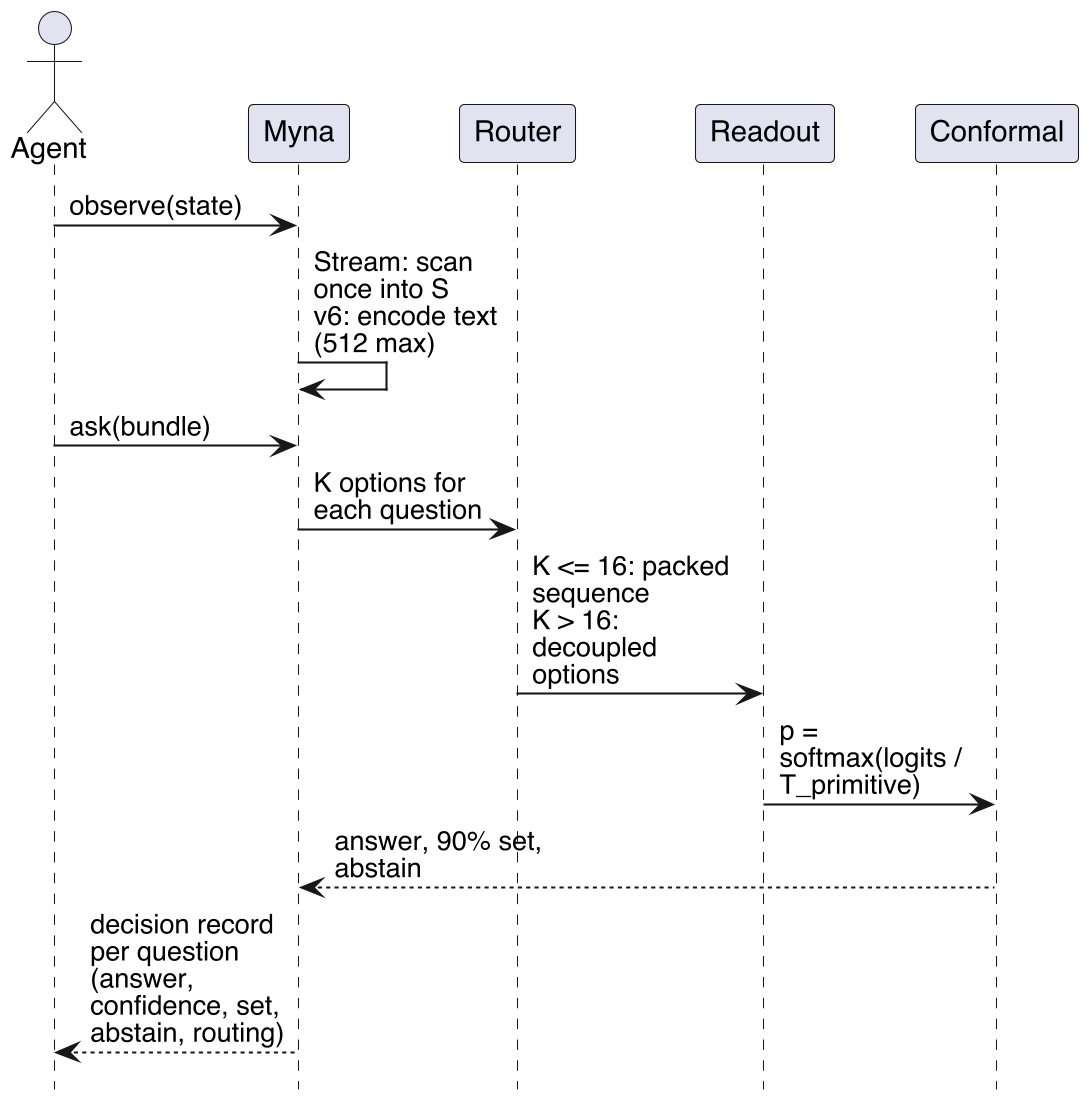
\includegraphics[width=0.72\linewidth]{fig7_sequence.png}
\caption{The \myna{} decision sequence for one bundle. The router chooses packed scoring for $K\le16$ and decoupled scoring for $K>16$; the conformal gate attaches a 90\% set and an abstention flag.}
\label{fig:sequence}
\end{widefigure}

\begin{widefigure}
\centering
\includegraphics[width=0.92\linewidth]{fig3_ablation.pdf}
\caption{(a) The two routing steps: v5 Packed 0.8173, v5 Unified 0.8502, v6 0.8583, and the local re-score 0.8620. (b) Per-cell accuracy change for each step. Every non-banking77 cell is 0.0000 in both steps; the aggregate gains are the 77-way cell divided by 16.}
\label{fig:ablation}
\end{widefigure}

\begin{widefigure}
\centering
\includegraphics[width=0.94\linewidth]{fig6_diagnostics_journal.pdf}
\caption{(a) Synthetic versus real-suite macro. The dashed line is the 0.94 synthetic gate; the dotted line is the 0.433 majority floor. The anti-prior arm removes four constant emitters and loses 0.0554 macro; the off arm is VOID. (b) Needle accuracy against state length for the 4k-trained arm: flat at the 0.167 floor.}
\label{fig:diagnostics}
\end{widefigure}

\end{document}
